%auto-ignore
%      this ensures the arxiv doesn't try to start TeXing here.
%!TEX root = super_lattice_models_draft.tex
%      prev line helps TeXShop do the right thing



%%%%%%%%%%%%%%%%%%%%%
 \section{Super pivotal Hamiltonian}
 \label{Super_pivotal_Hamiltonian}
 %%%%%%%%%%%%%%%%%%%%

In this section we will write down a commuting projector Hamiltonian 
for a generic fermionic topological phase. 
Since our goal in this section is to be rather general, we will put a fair amount of effort into making our construction 
mathematically precise -- readers who are only interested in the final result may skip to \ref{terms_in_Hamiltonian}. 

 \begin{figure}
\begin{center}
  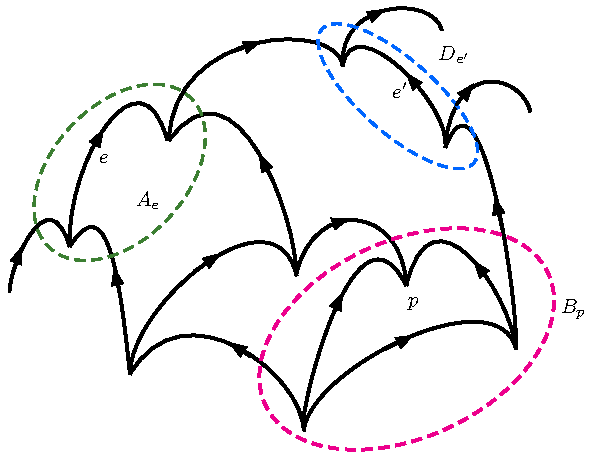
\includegraphics{sample_lattice.pdf}
 \caption{A cartoon of the support of the operators appearing in a super pivotal Hamiltonian on a section of a generic graph. 
The motivation for the strange-looking vertices is explained in Section \ref{standardized_handles}.
Dashed ellipses indicate the support of various terms in the Hamiltonian, on edges $e,e'$ and a plaquette $p$.
The vertex terms $A_e$ act on edges and project onto states with edge colorings that are consistent between adjacent vertices. 
The edge terms $D_e$ are responsible for sliding fermions along q-type edges. 
The plaquette terms $B_p$ involve all of the vertices and edges neighboring $p$.
They project onto graph configurations that contain no quasiparticles within the plaquette $p$.
\ethan{Dave may want to redo this figure}
\dave{at Dave's discretion.}
}
 \label{example_lattice}
 \end{center}
 \end{figure}

We will follow the same basic construction as in \cite{levin2005}, with modifications to take into account 
the fermionic nature of the phases under consideration. 
The most important modifications are as follows:
First, we will need to fix a spin structure on the manifold on which we are working.
This spin structure affects the details of the local projections which constitute the Hamiltonian, and is a necessary feature of any fermionic lattice model.
Additionally, we will need to allow the local degrees of freedom that constitute the 
Hilbert space for our lattice model to be super vector spaces, rather than the regular vector spaces in bosonic models. 
Finally, we will need to add a new term in the Hamiltonian with support on the edges and pairs of neighboring vertices in the lattice that allows fermions to fluctuate across edges 
that host q-type strings.

To begin the construction of the lattice model, we will thus need the following data:
\begin{enumerate}
\item a super pivotal fusion category ${\cal C}$,
\item a spin surface $\Sigma$,
\item and a graph $\mcg$ embedded in $\Sigma$ (more precisely, a cell decomposition of $\Sigma$) which inherits information about the spin structure.
\end{enumerate}
In the following subsections we define the Hamiltonian explicitly in terms of the above data.
%\kw{I think we should consider not using ``lattice", or at least being more careful with how we use it.
%For a mathematician, a lattice is a translationally-invariant structure on $\mathbb R^n$.}
%\ethan{Ah, good point. ``string-net graph''? ``Cell decomposition'' is also fine (I avoided this at first since most physicists won't have heard it before, but I don't think that matters too much).}
%\dave{I'm fine with not using lattice.
%I like the sound of ``string-net graph" but this may be a little confusing since it mixes the vector space with the lattice (which of course are related).
%I would also be fine with saying ``spin-graph", or ``super-graph", or ``super-spin-graph".
%Probably just ``graph" would do fine.
%}
%We will explicitly write out the Hamiltonian for the example of the honeycomb lattice shown in Fig.~\ref{example_lattice}, although much of what we say holds more generally.

We will write a frustration-free Hamiltonian as a sum of local projectors, which fall into
three classes.
Two of these classes of projector are the fermionic analogues of the plaquette and vertex terms from the usual Levin-Wen Hamiltonian, 
%\kw{should we cal it the Levin-Wen Hamiltonian, at least initially?  your call.}
%\dave{Lets call it the Levin-Wen Hamiltonian.
%I changed it.}
while the third is an edge term which allows fermions to fluctuate across edges hosting q-type strings.
The Hamiltonian takes the form
\begin{align} \label{ham}
H = \lambda_p \sum_{p \in \mcf} (1-B_p) + \lambda_e \sum_{e \in \mce} (1-D_e) + \lambda_v \sum_{e \in \mce} (1-A_e),
\end{align}
%\kw{I think there is some inconsistency about vertex terms; see nearby figure}
%\dave{Yes, definitely. 
%A very annoying issue. 
%One option is to keep it as $\sum_v A_v$ but have it supported on $v$ and all neighbouring vertices. 
%This has the benefiet of the vertex term being labeled by the vertices.
%Alternatively we could write it as $\sum_e A_e$, but this is somewhat displeasing. 
%Lets think if there is a comprimise between the two situations where we can (honestly) label the vertex term $A_v$.
%}
where the sums are over the plaquettes (faces) $\mcf$ and edges $\mce$ of the graph, 
%\ethan{we used mathcal stuff in the state-sum section, so I mathcalized the things to be consistent}
and the $\lambda_p,\lambda_e,\lambda_v$ are positive constants.
%We require a hierarchy in the couplings, $\lambda_p \ll \lambda_e \ll \lambda_v$,
%which ensures that the low energy spectrum can be characterized by simple objects in $\mcz(\mathcal{C})$.
%If we want the excitations to be in correspondence with the primitive idempotents of the tube algebra, then w
As in the bosonic case, we require a hierarchy in the couplings of $\lambda_v \gg \lambda_e \gg \lambda_p$\footnote{This makes the low energy spectrum consist purely of ``flux" excitations: 
the ``charged" idempotents always violate both the plaquette and $A_e$ term, which with this hierarchy of coefficients costs a large amount of energy. 
One way to put charge and flux excitations on an energetically more equal footing is to add ``tails'' to each 
plaquette that host the charge degrees of freedom, as in \cite{Hu2015}.
\dave{I vaguely remember Fiona Burnell also explaining this idea to me at one point, 
we should check and cite both.
I'll look into this soon.}
\dave{I will do this.}
Alternatively, we could modify the Hamiltonian so that $B_p \rightarrow B_p \prod_{e \in p} (1-D_e) \prod_{v \in p} (1-A_v)$, and $D_e \rightarrow D_e \prod_{v \in e} (1-A_v)$.
}.
%\dave{This makes the low energy spectrum purely ``flux" excitations. 
%The ``charged" idempotents always violate both the plaquette and vertex term, which with this hiearchy costs a lot of energy. 
%We could mention in a footnote that if this bothers the reader then the the plaquette term can be modified by $B_p \rightarrow B_p \prod_{v \in p} A_v$ or make the model an actual commuting projector Hamiltonian by taking $B_p \rightarrow B_p \prod_{e \in p} D_e \prod_{v \in p} A_v$, and $D_e \rightarrow D_e \prod_{v \in e} A_v$. }
%\kw{This is an issue for the usual bosonic LW Hamiltonian too.
%Is there anything we can refer to for the bosonic case?}
%\dave{Perhaps this one \cite{Hu2015}. 
%It looks like they circumvent the problem by adding an extra leg to the vertices to accomadate the flux+charge excitations.
%Ethan are you familiar with that paper? Or do you know if there are other appropriate references.}
%\kw{We should add a remark along the lines of Dave's suggestion.}
This is because the operators appearing in the plaquette terms are not well-defined unless the edge term energies are minimized, and in turn the terms appearing in the edge operators are not well-defined unless the terms involving $A_e$ are minimized.
Thus, the projectors associated with $k$-cells are only defined on the ground states of the projectors associated with $l$-cells, for all $l<k$.  
%\kw{maybe insert a caveat about later projectors only being defined on the ground state of earlier projectors}
%\ethan{I had a comment along these lines at a later point; moved it here instead}
%\dave{I changed ``commuting projector" to ``frustration free" above. 
%We should elaborate that when the vertex end edge terms the Hamiltonian is a commuting projector model.}
In Fig.~\ref{example_lattice} we illustrate the support of each operator appearing in the Hamiltonian with dashed circles, where we have drawn a section of the graph $\mcg$ embedded in the plane for the sake of visualization. 
For simplicity, we will assume that all vertices in $\mcg$ are trivalent\footnote{Any surface possesses a cell decomposition with trivalent vertices.
Such cell decompositions are Poincar\'e dual to triangulations.}.


\kwx{to do: Add (somewhere, not necessarily here) short remark about why the Hamiltonian is hermetian.}


%%%%%%%%%%%%%%%
\subsection{Hilbert space} \label{hilbertspacesect}
%%%%%%%%%%%%%%%

We will locate all all degrees of freedom (spins) at the vertices of the graph $\mcg$, so
the big Hilbert space on which the Hamiltonian is defined is
\begin{align}	\label{GraphHilbertSpace}
 \mch_\mcg =\bigotimes_{v \in \mcv} \mch_v.  %= \mch_{v_1} \tp \mch_{v_{2}} \tp \dots \tp \mch_{v_n} .
\end{align}
We are making use of the unordered tensor product defined in Section \ref{koszul_signs}.
%The tensor products above are supercommutative, 
%\kw{supercommutative is not the right adjective here; we need to find all other places in the paper where ``supercommutative" is used this way.
%Probably we should use the unordered tensor product (which incorporates Koszul signs).\dave{Agreed, modified.}}
%\dave{
%The other places we use supercommute are the introduction, 
%and the appendix on basic facts about super algebras.
%The context is `tensor product of morphisms supercommute' (maybe should be changed to `super interchange law') and 
%`elements of an algebra can super commute' (I think this is the correct context).
%}
%in the sense that for $\psi\in \mch_{v_i},\eta\in \mch_{v_{i+1}}$, $\psi \tp \eta = (-1)^{|\psi||\eta|}\eta\tp\psi \in \mch_{v_{i+1}} \tp \mch_{v_i}$. 

The vertex Hilbert spaces $\mch_{v}$ will depend on three sets of choices.
First, we must choose an orientation of each edge of $\mcg$.
This is because of the possibility of non-trivial Frobenius-Schur indicators; see below.
Second, we must choose an ordering of the edges incident to each vertex, consistent with with the intrinsic cyclic ordering of those edges
coming from the embedding of $\mcg$ in the oriented surface
(so if the vertex is $r$-valent, there are $r$ possible orderings).
Finally, we must choose a spin framing at each vertex.

In order to make the choice of cyclic ordering manifest in diagrams, and in order to simplify spin-structure-related
aspects of our construction, we will choose to draw our graphs in a way such that all of the 
edges at each trivalent vertex are ``on the same footing''. This is in contrast to the conventions in the physics literature
and in the earlier sections of this paper, where vertices are drawn with one edge extending below the vertex and two 
edges extending above, since in this convention the edge extending below is distinguished from the two other edges.
We will choose a convention in which all three edges at each trivalent vertex extend above the vertex: with this
choice, each vertex resembles a pitchfork. 
%The cyclic ordering of the edges at a given vertex is determined by the left-to-right ordering of the pitchfork legs. 

We must also choose a spin framing at each vertex, consistent with the ``pitchforkization'' convention.
The pitchforkization and spin framing are needed in order to define an unambiguous
isomorphism between local degrees of freedom at $v$ is standard vector spaces $V^{abc}$.
Without this standardization, the local Hilbert spaces would be ambiguous up to automorphisms. 
The standardization procedure is nothing more than fixing a convenient choice of gauge in the way we present our fusion diagrams. 

If all the edges incident to a vertex $v$ point out of the vertex, we define the vertex Hilbert space at $v$ by 
\be
	\mch_v = \bigoplus_{a,b,c} V^{abc}  \quad\quad\quad\quad\quad\quad \PitchFork{a}{b}{c}{},
	\label{pitchfork_basis}
\ee
where the sum is over the simple objects of $\spc$.
%\footnote{We choose our favorite complete set of representatives of isomorphism classes of simple objects $\sob(\spc)$ at the outset and keep it fixed throughout, abusing notation slightly by writing $\spc$ for $\sob(\spc)$.
%\kw{I don't see where we are abusing notation like this}
%\ethan{right. This footnote was written when we were, but then we changed our ways and started using $\sob(\spc)$ for everything. Commented out the offending footnote.}}.
%where the sum is over the simple objects of $\spc$\footnote{We choose our favorite complete set of representatives of isomorphism classes of simple objects $\sob(\spc)$ at the outset and keep it fixed throughout, abusing notation slightly by writing $\spc$ for $\sob(\spc)$.
%\kw{I don't see where we are abusing notation like this}
%\dave{This section probably predates the $\sob(...)$ notation.
%Lets remove the footnote and make sure we don't have any $\sum_{x \in \spc/\psi}$ etc. left over.}
%\ethan{right. I wrote the footnote when we were, but then we changed our ways and started using $\sob(\spc)$ for everything (which is better).}}.
If the first edge points in and the other two point out, then we define
\be
	\mch_v = \bigoplus_{a,b,c} V^{a^*bc}  \quad\quad\quad\quad\quad\quad \PitchForkas{a}{b}{c}{} =  \PitchFork{a^*}{b}{c}{},
\ee
and so on for all eight possible patterns of in/out of the three incident edges.

\medskip

This completes the definition on the big Hilbert space for the Hamiltonian.
Impatient readers should now skip to the next subsection, but readers who are puzzled by some of the choices we made above 
are encouraged to read on.

\medskip

Why are there no spins on edges, as in the original Levin-Wen Hamiltonian?
Levin and Wen explicitly assume that $V^{abc}$ is at most 1-dimensional.
This is true for theories based on Temperley-Lieb or $Rep_q(sl_2)$, but it is not true in general,
so we need to add spins on vertices.
But each basis vector in $\bigoplus_{a,b,c} V^{abc}$ ``knows" the labels on the adjacent edges, so once we have these vertex degrees of
freedom the edge degrees of freedom become redundant and can be eliminated\footnote{An argument in favor of edge degrees of freedom is that they can lead to smaller local Hilbert spaces, at least for simple theories.
For example, one can write a Hamiltonian for the $C_2$ theory which has a $(2|0)$-dimensional Hilbert space at each edge
and a $(1|1)$-dimensional Hilbert space at each vertex.
The general Hamiltonian we are now discussing, specialized to the $C_2$ theory, 
would assign a $(4|3)$-dimensional Hilbert space to each vertex (but no Hilbert spaces for edges).}.

Why must we choose an orientation of each edge?
The short answer: because of the possibility of non-trivial Frobenius-Schur indicators.
Now for the longer answer.
If the edges are not oriented, then we would assign vertex Hilbert spaces as above, but with all edges point out at each vertex.
This means that each edge sees two inward pointing edges.
\begin{align}
\PitchForkWithEdge
\end{align}
If the two labels coming from the two adjacent vertices are $a$ and $b$
(which we will assume are both m-type, for simplicity), then the
associated vector space for the edge is $V_{ab}$, which is 0-dimensional unless $a \cong b^*$.
If $a$ is not self-dual, or if $a$ is evenly self-dual with FS indicator 1, then there is a canonical identification of $V_{ab}$ with 
$\cc = \cc^{1|0}$ and we can ignore it.

But if $a$ is evenly self-dual with FS indicator $-1$, then there is a sign ambiguity in identifying $V_{aa}$ with $\cc$, and we will have to
keep careful track of this sign when defining the Hamiltonian.
Even worse, if $a$ is {\it oddly} self-dual (and $a$ is m-type), with FS indicator $\pm i$ (as occurs in the $\halfesix$ theory studied earlier), then $V_{aa}$ is an odd vector space, 
non-canonically isomorphic to $\cc^{0|1}$.
Keeping track of these odd vector spaces would entail even more bookkeeping.

Overall, we think the least annoying solution to the above problems is to orient each edge of the graph.
This allows us to treat $a$ and $a^*$ as distinct objects, even when they happen to be isomorphic.
Now, instead of $V_{aa}$, we have $V_{aa^*} \cong \End(a)$, which has a canonical element $id: a\to a$,
even when Frobenius-Schur indicators are nontrivial.

Why the pitchforks? As alluded to earlier, rotations by $2\pi/3$ can act non-trivially on $V^{aaa}$, and so it is helpful to choose a vertex configuration where every outgoing edge is placed on the same footing. 
This is true even in the bosonic case.

Why the spin framings?
Because $V^{abc}$ has a spin-flip automorphism, and also because we need to 
enhance the graph $\mcg$ with information related to the spin structure of the ambient manifold 
in order to write the edge terms, as explained below.










%%%%%%%%%%%%%



%%%%%%%%%%%%%%%%%%%%
%%%%%%%%%%%%%%%%%%%%



%%%%%%%%%%%%%%%%%%
\subsection{Spin structure considerations and the standardization of the graph} \label{standardized_handles}
%%%%%%%%%%%%%%%%%%


To derive the Hamiltonian \eqref{ham} and explain the nature of the $B_p$, $D_e$, and $A_v$ operators, we will first need to describe how the graph inherits spin structure data from the ambient spin manifold on which it is defined. 

Recall that we have a graph $\mcg$ embedded in an orientable spin surface $\Sigma$.
In order to define the super pivotal Hamiltonian we will need to equip $\mcg$ with information about the spin structure $\sigma$. 
In order to talk about the spin structure data at the vertices and edges of $\mcg$, we will thicken the cell decomposition to a handle decomposition of $\Sigma$.
A handle decomposition is essentially a fattened version of a graph; see Fig.~\ref{HandleDecomposition} for an illustration.
\begin{figure}
  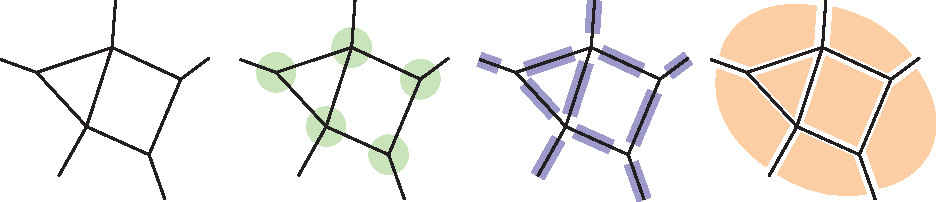
\includegraphics{HandleDecomposition.pdf}
  \caption{A handle decomposition obtained from the graph on the far left.
  The $0$ handles (green disks) are neighborhoods of the vertices, the $1$-handles (purple strips) are neighborhoods of the edges, 
%  \kw{purple 1-handles should not intersect the 0-handles except at their boundary; need to shrink them a bit.}
  %\dave{I will fix this.}
  and the $2$ handles (orange polygons) which are the compliment of the union of the $0$- and $1$-handles.}
  \label{HandleDecomposition}
\end{figure}
The handle decomposition can be obtained by expanding each vertex of the graph into a disk ($0$-handle) and each edge into
a thickened strip (1-handle).
The remaining faces constitute the $2$-handles, which are homeomorphic to disks.

Recall from Section \ref{hilbertspacesect} that 
in order to define the local vertex degrees of freedom we choose an orientation for each edge, a ``pitchforkization" for each vertex, and a spin framing at each vertex.
These choices are analogous to choosing a gauge -- different choices lead to isomorphic Hamiltonians and ground states.


The choices of pitchforkization and spin framing are equivalent to choosing a spin diffeomorphism from a 0-handle to a standard model for a 0-handle.
We define a spin diffeomorphism $\varphi_v$ from a generic 0-handle $v$ to a disk in $\rr^2$ with its standard spin structure, so that the attaching regions for the 1-handles terminating on $v$ are all located on the top part of the disk. 
%\footnote{Note that there is a large degree of gauge freedom in this construction, realized by performing $2\pi$ rotations of the fermion framing (spin flips) on the spin diffeomorphisms $\varphi_v$.}
That is, we use the spin diffeomorphisms to turn each 0-handle into a ``standardized 0-handle'', where the configuration of the 1-handles terminating on each 0-handle means that that each 0-handle looks like a pitchfork.
The spin diffeomorphism $\varphi_v$ that maps a generic 0-cell $v$ to a standardized 0-cell (thereby implementing the pitchforkization procedure) is defined pictorially by
%\dave{Will add `directions' to each edge.}
\begin{align} \label{std0handle}
\xymatrix @!0 @M=1mm @R=14mm @C=35mm{
 \varphi_v: \; \; D_v\ar[r]            & D(n) \\
\;\;\;\;\;\;\; \Dv \ar@{|->}[r] & \Dfv
	} 
\end{align} 
where $n$ is the number of edges which terminate at $v$ and the black arrow in the picture on the right hand side denotes the fermion framing of the 0-handle, which is constant throughout the 0-handle.  
When writing down the Hamiltonian we always take $n=3$ without loss of generality, but when discussing tensor network constructions of these phases it is helpful to let $n$ be unspecified. 
Using the pitchforkization map $\varphi_v$ 
we can pull back the standard spin framing of $\rr^2$ to the 0-handle.
This results in a spin framing which is parallel to the outgoing edges at the top of the 0-handle. 

\begin{figure}\centering{
  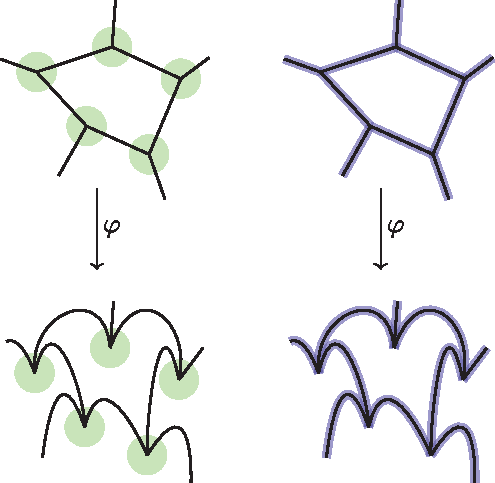
\includegraphics{SpinIsomorphisms.pdf}}
  \caption{The mapping $\varphi$ that maps a generic handle decomposition (top row) onto a ``standardized'' handle decomposition in which each 0-handle (green disk) has an identical pitchfork configuration (bottom row).
%  \dave{Need to fix figure.}
    }
  \label{SpinIsomorphisms}
\end{figure}

Just as we do for the 0-handles, we will ``standardize'' the 1-handles so that they all assume the same form. 
After standardizing our 0-handles, 1-handles will always enter/exit from a 0-handle ``vertically'' (see Figure \ref{SpinIsomorphisms}), 
and so our standardized 1-handles will look like 
\begin{align}
\Horseshoe
\end{align}

For theories with q-type particles, the Hamiltonian will contain terms that allow fermions to fluctuate across a 1-handle from vertex to vertex. 
The spin structure on a 1-handle (relative to the two attaching intervals) will determine what phase factor a fermion picks up when it moves across a 1-handle. 

\begin{figure}
\begin{center}
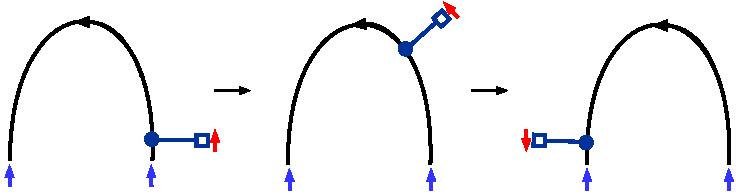
\includegraphics{framing_rotation.pdf}
\end{center}
\caption{\label{framing_rot} Parallel-transporting a fermion along a q-type edge, which is oriented as shown. 
The red arrow keeps track of the fermion framing, which rotates by $\pi$ when proceeding along the direction of the edge's orientation.
The blue arrows at the ends of the edge indicate the fixed framing at each 0-handle at the endpoints of the edge. 
}
  \label{framing_rotation}
\end{figure}

Once we have chosen coordinates at each vertex, we can associate a spin rotation of $+\pi$ or
$-\pi$ to each 1-handle.
First, we choose a standard spin framing at the incoming side (recall that each edge is directed) of the 1-handle.
A standard choice exists because we have chosen a standard spin framing for the 0-handle at the incoming end of the 1-handle. 
We then parallel transport the spin framing along the 1-handle, keeping the first basis vector of the spin framing tangent to 
the core of
the 1-handle during the transporting process.
This procedure is illustrated in Figure \ref{framing_rotation}, where the red arrow denotes the first basis vector of the spin framing. 
When we arrive at the end of the 1-handle, the spin framing we have transported will not agree with the standardized spin framing at the second 0-handle. 
We can see this from Figure \ref{framing_rotation}; we have chosen the spin framing to point upwards at each 0-handle, but the red arrow points downward when it reaches the end of the 1-handle, which disagrees with the framing at the 0-handle. 
These two framings are related by either a $+\pi$ or $-\pi$ spin rotation in $Spin(2)$.
\begin{figure}
\begin{center}
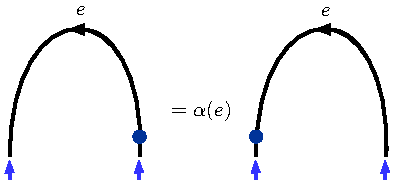
\includegraphics{alphae_defn.pdf}
\caption{\label{alphae_defn} The action of sliding a fermion across an edge $e$ labeled by the q-type object $b$ is given by $\alpha(e,b)$. 
The spin framings of the 0-handles on either end of $e$ are denoted by the blue arrows, 
and  the spin framing of the fermion on the right hand side is taken to match that of the left 0-handle. }
\end{center}
\end{figure}
We will denote this element of $Spin(2)$ by $\alpha(e)$, where $e$ is the edge corresponding to the 1-handle.

Note that the collection $\{\alpha(e)\}$ is determined by the the spin structure of $\Sigma$ and
the choice of spin framings at each 0-handle.
Conversely, any collection $\{\alpha(e)\}$ determines a spin structure on $\Sigma\setminus\{\mbox{2-handles}\}$.
In order for this spin structure to extend to all of $\Sigma$, $\{\alpha(e)\}$ must satisfy the constraint that the 
boundary of each 2-handle has a bounding spin structure; see below.

Let $b$ be a q-type simple object.
We want to analyze the effect of sliding a fermionic dot over the edge $e$ when $e$ is labeled by $b$.
At the outset, we will choose an odd element $\gamma_b\in\End(b)$ such that $\gamma_b^2 = \id_b$, and also
$\gamma_{b^*}\in\End(b^*)$ such that $\gamma_{b^*}^2 = \id_{b^*}$.
The requirement that $\gamma_b^2 = \id_b$ determines $\gamma_b$ up to sign.
Let $r(b)\in\cc$ be such that $R_\pi\cdot\gamma_b = r(b)\gamma_{b^*}$, where
\be
	R_\pi : \End(b) \to \End(b^*)
\ee
denotes the spin rotation by $+\pi$.
It is easy to see that $r(b) = \pm i$.
The exact value will depend on the choices of standard generators $\gamma_b$ and $\gamma_{b^*}$.
If $b$ is not isomorphic to $b^*$, then we can always choose $\gamma_b$ and $\gamma_{b^*}$ so that $r(b) = i$.
But if $b = b^*$ (as happens in the $C_2$ theory, for example), then $\gamma_b = \gamma_{b^*}$ and the value of $r(b)$
is forced upon us, independent of the choice of $\gamma_b$.\footnote{
The condition that $b$ is equal to, rather than merely isomorphic to, $b^*$ is in some sense pathological.
But for theories build out of unoriented strands, like $C_2$, it is convenient to allow this pathology.}

We can now, finally, describe the effect of sliding a standard fermionic endomorphism (dot) over an edge $e$ labeled by 
a q-type particle $b$.
Let $\gamma_b * e$ denote the edge with the standard generator $\gamma_b$ placed at the incoming end (left side of Figure \ref{alphae_defn}).
Let $e* \gamma_{b^*}$ denote the edge with the standard generator $\gamma_{b^*}$ placed at the outgoing end (right side of Figure \ref{alphae_defn}).
Then
\be
	\gamma_b * e = \alpha(e, b) \cdot e* \gamma_{b^*} ,
	\label{fermion_slide}
\ee
where
\be
	\alpha(e, b) =  \left\{   \begin{array}{ll}  
		r(b) & \mbox{if $\alpha(e) = R_\pi$} \\
		-r(b) & \mbox{if $\alpha(e) = R_{-\pi}$} \\
	\end{array}  \right. .
\ee
This is illustrated in Figure \ref{alphae_defn}.

%\kw{should probably move definition of $\Gamma$ to definition section} 
%\ethan{we already kinda do with our discussion of displacing dots onto edges. maybe I can try to just expand that discussion}
Fermionic dots can also be ``absorbed'' into vertices using the action of $\cliff_1$ on 
fusion spaces involving q-type objects, as discussed in Section \eqref{fusion_spaces}. 
We can do this in analogy with \eqref{Gamma_y_def} by constructing odd operators $\Gamma_i$, $i\in \{1,2,3\}$, which map a pitchfork with a standard dot 
on the $i$-th outgoing pitchfork edge to a pitchfork without a fermion dot on the $i$-th leg. 
Graphically, $\Gamma_1$ is defined by 
\be \label{gamma1_defn}
\underset{\psi}{\Pitchforkdotone} = \sum_{\eta}[ \Gamma_1 ]_{\psi \eta} \underset{\eta}{\PitchforkLarge}
%\mathord{\vcenter{\hbox{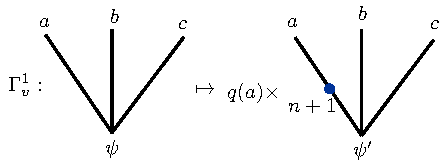
\includegraphics[scale=1]{Gamma1def.pdf}}}},
\ee
where $\psi,\eta$ are basis vectors for $V^{abc}$, and the fermionic dot has a higher sign ordering than the basis vector it sits on.
%in the fusion space of the pitchfork for a fixed coloring of the pitchfork's outgoing legs. 
$\Gamma_2$ and $\Gamma_3$ are defined similarly:
\footnote{\dave{dave will make this more correct.}
The matrix elements of $\Gamma_1$ can be written in terms of net evaluations as $[\Gamma_1]_{\psi \eta}  ={\BananaDot} \left(  \Bananaeta \right)^{-1} $, and similarly for 
$\Gamma_2$ and $\Gamma_3$. }
\be \label{gamma2gamma3_defn}
\underset{\psi}{\Pitchforkdottwo} = \sum_{\eta}[ \Gamma_2 ]_{\psi \eta} \underset{\eta}{\PitchforkLarge}, \quad \quad
\underset{\psi}{\Pitchforkdotthree} = \sum_{\eta}[ \Gamma_3 ]_{\psi \eta} \underset{\eta}{\PitchforkLarge}
%\mathord{\vcenter{\hbox{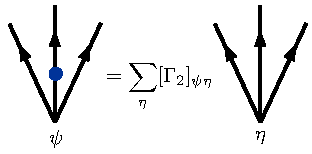
\includegraphics[scale=1]{Gamma2def.pdf}}}},
%\quad
%\mathord{\vcenter{\hbox{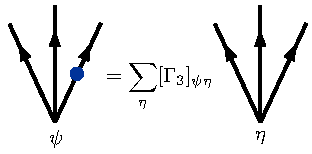
\includegraphics[scale=1]{Gamma3def.pdf}}}},\quad
\ee
%\kw{We could move this to the definition section, and if we do that then we could keep it here too or delete it here.}
Since only q-type objects can host fermionic dots, $\Gamma_i$ is only defined when the $i$-th 
leg of the vertex is labeled by a q-type object. 
%The $\Gamma_i$ are all odd matrices, reversing fermion parity.
%\dave{It probably makes sense to put it in the definition section, but I have no strong preference.
%In the definition section we already have the non pitchfork version of it defined.}
%\ethan{It is slightly redundant to have it here, but I am in favor of keeping it---I think it's nicer to leave the few lines here and save the reader the trouble of flipping back to the definition section for stuff}
Since only q-type objects have odd endomorphisms, 
$\Gamma_i$ is only defined when the i-{th} label of the pitchfork is q-type.
%Since only q-type particles can host fermionic dots, we set $\Gamma_i=0$ unless the $i$th leg is colored by a q-type object. 
The $\Gamma_i$ are all odd matrices, reversing fermion parity.

%%KW the remark about sigma^x seems confusing and unnecessary to me.
%The $\Gamma_i$ are all odd matrices, meaning that they act as $\sigma^x$ on the fermion parity grading in a representation where $(-1)^F$ acts as $\sigma_z$.
%For more complicated theories, they will also act nontrivially on the multiplicity degrees of freedom by the action of 
%some unitary matrix (e.g.\ equation \eqref{esixdotslide} for the $\halfesix$ theory). 


%\kw{I think we should drop this paragraph.}
%it got turned into a footnote
%The matrix elements of the $\Gamma_i$ matrices for a fixed coloring $a,b,c$
%of the legs of a given vertex can be written in terms of evaluated diagrams 
%by using the inner product \eqref{reflection_pairing_defn} on pitchforks, which allows us to evaluate 
%vectors in $V^{abc} \tp V^{c^*b^*a^*}$.
%Denoting the dual of a vector $\psi\in V^{abc}$ by $\psi^*$ so that 
%$\mcb(\eta\tp\psi^*)\propto\delta_{\eta,\psi}$, we can write 
%\begin{align}
%[\Gamma_1]_{\psi \eta}  ={\BananaDot} \left(  \Bananaeta \right)^{-1} 
%\end{align}
%\be \mathord{\vcenter{\hbox{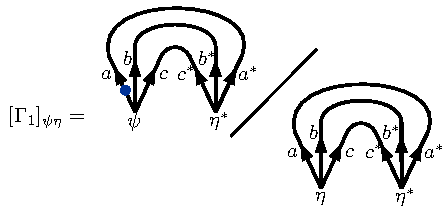
\includegraphics[scale=1]{gamma1_matrix_elements.pdf}}}}, \ee
%and similarly for $\Gamma_2$ and $\Gamma_3$. 

\dave{Will either delete or substantiate.}
It is easy to check that when they are non-zero (i.e.\ when they act on q-type edges), the $\Gamma_i$ operators obey the anti-commutation relations 
\be \{ \Gamma_i , \Gamma_j \} = 2\lambda \delta_{ij},\ee
which are the defining relations for the representations of complex Clifford algebras, and where as before, $\lambda=\pm i$ is the phase picked up when removing a pair of dots from a q-type object worldline. 


\medskip

\begin{figure}
\begin{center}
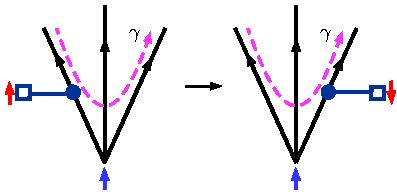
\includegraphics{spin_rot_through_0handle.pdf}
\caption{ \label{spin_rot_through_0handle} An illustration of a $+\pi$ spin framing rotation picked up as the path $\gamma$ (drawn in dashed purple) passes through a 0-handle. 
If we were to proceed along $\gamma$ in the opposite direction, we would pick up a $-\pi$ spin framing rotation instead.   }
\end{center}
\end{figure}

We mentioned above that the collection of $\{\alpha(e)\}$ must satisfy some constraints if it is 
to extend over the 2-cells and give a specified spin structure.
Here are the details:
let $\gamma$ be an oriented framed loop in $\Sigma$.
For simplicity, we will assume that (a) $\gamma$ is embedded, (b) the framing is the natural one coming from the tangent 
space of $\gamma$, and (c) $\gamma$ is contained in the union of the 0- and 1-handles.
We want to compute the spin rotation, either 0 or $2\pi$, which $\gamma$ picks up from the spin structure on the 0- and 1-handles.
When $\gamma$ goes over a 1-handle $e$, it picks up a rotation of $\alpha(e)$ or $-\alpha(e)$, depending on whether it goes over $e$
with or against the orientation of $e$.
Each time $\gamma$ passes though a 0-handle, it also picks up a rotation of $\pm\pi$.
Suppose $\gamma$ enters the 0-handle at the $i$-th 1-handle and exits the 0-handle at the $j$-th 1-handle\footnote{Note that $i$ and $j$ refer to the ordering of 1-handle attachments local to the 0-handle, not to some global ordering. The $i$ and $j$ are assigned in the same way as the $\Gamma_i$ and $\Gamma_j$ in \eqref{gamma1_defn} and \eqref{gamma2gamma3_defn}.}.
With our ordering conventions, this gives a rotation of $+\pi$ if $i<j$ and a rotation of $-\pi$ if $i > j$ (see Figure \ref{spin_rot_through_0handle}).
Combining all of these $\pm\pi$ rotations results in a rotation of 0 or $2\pi$.
A bounding spin structure on $\gamma$ yields a $2\pi$ rotation (since a $2\pi$ rotation acts as 
multiplication by $-1$ and produces the requisite anti-periodic boundary conditions), and a non-bounding 
spin structure corresponds to no rotation.
In particular, if $\gamma$ is the boundary of a single 2-cell/plaquette, then it must correspond to a spin 
framing rotation of $2\pi$, since we assume that the spin structure around each 2-cell is bounding (which 
allows the spin structure on the 0- and 1-handles extends to a spin structure on all of $\Sigma$). 
More generally, $\gamma$ will always get a spin framing rotation by $2\pi$ if it is in the trivial homology 
class of $H_1(\Sigma)$.



%%%%%%%%%%%%%%%%%%%%%
\subsection{Terms in the Hamiltonian} \label{terms_in_Hamiltonian}
%%%%%%%%%%%%%%%%%%%%%

In this section we will finally write down the Hamiltonian, and then explain the terms appearing in it in detail. 
As mentioned earlier, the Hamiltonian consists of three kinds of mutually commuting projections:
\begin{align} \label{terms_in_ham}
H = \lambda_p \sum_{p \in \mcf} (1-B_p)  + \lambda_e \sum_{e \in \mce} (1-D_e) + \lambda_v \sum_{e\in \mce} (1-A_e)
\end{align}
%\kw{probably need to index the ``vertex" terms by edges}
We'll start with a discussion of the ``vertex'' term $A_e$ and then address the new edge term $D_e$, 
finally ending by describing the plaquette term $B_p$.




%%%%%%%%%%%%%%%%
\subsubsection{Vertex term}   \label{VertexHamiltonian}
%%%%%%%%%%%%%%%%

Let $v_1$ and $v_2$ be two vertices joined by an edge $e$.
We define
\begin{align}
A_e(\ket{\psi_1} \otimes \ket{\psi_2}) = 
\left\{
                \begin{array}{ll}
                   \ket{\psi_1} \otimes \ket{\psi_2} & \text{if $\psi_1$ and $\psi_2$ assign the same label to $e$} \\
                  0 & \text{otherwise}
                \end{array}
              \right.
\end{align}
In other words, $A_e$ forces the labels on each end of an edge to agree.

Why do we call these ``vertex terms" when they are indexed by edges, and the support is a pair of adjacent vertices, joined by an edge?
Because it does the same work as the vertex term of the usual bosonic LW Hamiltonian.
If our fermionic category happens to be bosonic (i.e.\ it lacks fermions), then the ground state of our ``vertex" term is isomorphic to the ground state
of the vertex term in the usual LW Hamiltonian.\footnote{Note that the ``admissibility'' condition that requires $V^{abc}$ to be in the ground state vector space only if $\unit\in a\tp b \tp c$ is already satisfied for us, since our local Hilbert spaces at the vertices already have this condition built in.}
If we had chosen to put spins on edges as well as vertices, then we could write a vertex term that was actually indexed by vertices.
But its ground state would be isomorphic to the above edge-like vertex term.

Note that vectors in the ground state of the vertex term can be interpreted as string nets.
If $K$ is the ground state of the vertex term, we have maps
\be
	K \to \mch(\Sigma \setminus \mbox{2-cells}) \to \mch(\Sigma) .
	\label{ground_state_projection}
\ee
where $\mch(\Sigma \setminus \mbox{2-cells})$ and $\mch(\Sigma)$ are the ground-state Hilbert spaces of $\Sigma \setminus \mbox{2-cells}$ and $\Sigma$, respectively.
The job of the edge term (below) will be to pick out a subspace of $K$ on which the first map is an isomorphism. 
The job of the plaquette term will be to further reduce to a subspace such that the composite map to $H(\Sigma)$ is an isomorphism.




%%%%%%%%%%%%%%%%%%%%
\subsubsection{Edge term} 
\label{edge_term}
%%%%%%%%%%%%%%%%%%%%

The edge terms are the qualitatively new feature of this Hamiltonian, and are a necessary ingredient for the Hamiltonian of any theory possessing q-type particles. 
They are only well-defined on ground states of the vertex term. 
They allow fermions to fluctuate across edges of the graph which are labelled by q-type particles,
and provide a way of energetically implementing the isotopy relations associated with sliding fermions along the worldlines of q-type particles. 
In Section \ref{modified_tensor_product} we solved the same problem in
a different context by replacing a tensor product over scalars with a tensor product
over the endomorphism algebra of a q-type simple object.
The edge term of the Hamiltonian is a stand-in for the tensor product over a non-trivial endomorphism algebra.
%Implementing these isotopy relations can be done in two ways. 
%One is to add the edge term to the Hamiltonian which allows fermions fluctuate between vertices connected by a q-type edge, while another is to modify the tensor products appearing in the definition of $\mch_\mcg$ to be tensor products in which the algebra we're tensoring over is
%chosen from the endomorphism algebras of the edge labels. 
%We will describe the edge term approach in this section, and will address the latter method in Section \ref{modified_tensor_product}. 



The edge term will coherently add and remove fermions at the end points of the q-type bonds, as well as tunnel them across.\footnote{Heuristically we can think of two adjacent vertices as islands which can hold a number of fermions and whose fermion parity is well defined. 
If these vertices are connected by a q-type edge, we can think of that edge as a 1D superconductor which coherently couples the two islands together.}
This term favors an equal-weight (meaning equal up to a phase factor) 
superposition of fermions across all vertices connected by 
q-type simple objects with a fixed fermion parity.
Since the edge term is responsible for allowing fermions to fluctuate (``hop'') across edges labeled by q-type objects, 
it will be absent in any theory with no q-type objects.

Fermion hopping across q-type edges is implemented by the $\Gamma$ operators. 
To do this for an edge $e$, we can create a pair of fermions near the vertex at the beginning of $e$, slide one of the fermions along $e$ to the vertex at the end of $e$, and then use the $\Gamma$ operators to ``absorb'' each fermion into their respective vertices. 
For example, if $e$ hosts a q-type edge label $x$, then we have 
\begin{align}
\xymatrix @!0 @M=1mm @R=18mm @C=30mm{
\Edgea\ar[rr]^{\lambda^{-1}}&&\Edgeb\ar[dd]^{\alpha(e,x)} \\
&&\\
\Edgea&&\ar[ll]_{\Gamma_3 \tp \Gamma_1} \Edgec
	} 
	 \label{dot_slide_gamma} 
\end{align}
%\be \label{dot_slide_gamma} \mathord{\vcenter{\hbox{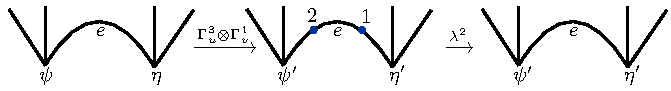
\includegraphics[scale=1]{dot_slide_gamma.pdf}}}},\ee
where we have defined tensor products of $\Gamma$ operators to act so that operators located further to the left in tensor products absorb fermions with higher order than the operators to their right.
Note that although the diagrams in the first and last steps in the above sequence look the same, they are not: the fermion parity of the vectors in the two vertex Hilbert spaces $V^{abx^*}$ and 
$V^{xcd}$ has been switched. 

%%%%
For a generic edge $e$ oriented from $v_1$ to $v_2$ and colored by a fixed object $x$ the edge term
can be written as the projector
\begin{align}
D_e = \frac{1}{2}(1+J_e),
\end{align}
where $J_e$ acts on vectors $|\psi_1\rangle \tp |\psi_2\rangle \in \mch_{v_1}\tp \mch_{v_2}$ 
by implementing the local relations coming from $\End(x)$:
\be J_e(|\psi_1\rangle\tp |\psi_2\rangle) = 
\begin{cases}
  \lambda^{-1}\alpha(e,x)\sum_{\eta_1,\eta_2}[\Gamma_i]_{\psi_1\eta_1} |\eta_1\rangle \tp [\Gamma_j]_{\psi_2\eta_2}|\eta_2\rangle \quad &\text{if $x$ is q-type}\\ 
 |\psi_1\rangle\tp |\psi_2\rangle \quad &\text{if $x$ is m-type} \end{cases}
\ee
Here, we have taken $e$ to be the $i$th leg of the pitchfork at $v_1$ and the $j$th leg at $v_2$, and $|\eta_1\rangle \tp |\eta_2\rangle \in \mch_{v_1} \tp \mch_{v_2}$.
Since $D_e$ acts as the identity on edges colored by m-type objects, edges with m-type edges will automatically lie in the ground state of the edge term. 
%%%%

%\dave{Old paragraph:
%In general, if $e$ is oriented from $v_1$ to $v_2$ colored by a fixed object $x$ and $|\psi_1\rangle \tp |\psi_2\rangle$ is a vector in $\mch_{v_1}\tp \mch_{v_2}$, the edge term $D_e$ acts as 
%\be D_e(|\psi_1\rangle\tp |\psi_2\rangle) = \begin{cases}
%  -\lambda\alpha(e,x)\sum_{\eta_1,\eta_2}[\Gamma_i]_{\psi_1\eta_1} |\eta_1\rangle \tp [\Gamma_j]_{\psi_2\eta_2}|\eta_2\rangle \quad &\text{if $x$ is q-type}\\ 
% |\psi_1\rangle\tp |\psi_2\rangle \quad &\text{if $x$ is m-type} \end{cases}
%\ee
%\kw{q-type line should be replaced by id - J, where J is the current RHS.  Probably define J (or whatever we call it) on a separate line.}
%\dave{Yeap.}
%where $e$ is the $i$th leg of the pitchfork at $v_1$ and the $j$th leg at $v_2$, and $|\eta_1\rangle %\tp |\eta_2\rangle \in \mch_{v_1} \tp \mch_{v_2}$.
%Since $D_e$ acts as the identity on edges colored by m-type objects, edges with m-type edges will automatically lie in the ground state of the edge term. 
%}

In summary, including $D_e$ in the Hamiltonian provides a way of energetically enforcing the conditions that the ground states of theories containing q-type particles are realized by superpositions of string-net configurations possessing all possible ways of arranging fermions on the q-type strings. 
Ensuring that ground states are superpositions of different fermion configurations is tantamount to projecting from the Hilbert space $\mch_\mcg$ to the physical Hilbert space $\mch_{\rm phys}$, in which redundant degrees of freedom created by different fermion configurations are modded out.


As mentioned earlier, it can be conceptually helpful to note that a 1D Kitaev wire in the topological phase also exhibits the same behavior as the q-type strings in our theories.
However, since generic theories (like the $\halfesix$ example considered earlier) can have fusion rules in which two q-type simple objects to fuse to a third q-type simple object, this analogy is not perfect, since at the junction of three Kitaev wires a zero mode is left behind, which does not occur in the $\halfesix$ theory. 
%\dave{I think we should be careful in saying that they are more general Kitaev wires.
%But lets Skype about this sometime.}

%%%%%%%%%%%%%%%%%%%%%%
%%%%%%%%%%%%%%%%%%%%%%




%%%%%%%%%%%%%%%%%
\subsubsection{Plaquette term}
%%%%%%%%%%%%%%%%%

As with the vertex term, the plaquette term is essentially the same as the plaquette term in the usual string-net Hamiltonian: 
it inserts an $\omega$ loop 
%loops labeled by different objects in $\spc$ 
into each plaquette, and uses local relations to fuse these $\omega$ loops into the boundaries of the plaquettes. 
Physically it is responsible for the dynamics of net configurations which reside in the ground space of the vertex and edge terms, 
and it is designed so that two string nets that correspond to the same state vector receive the same amplitude. \ethan{or something like that}
%It is responsible for the dynamics in the string-net phase, and allows us to perform time evolution on string-net states.  
%It is designed so that the amplitude of a net configuration is given by the evaluation of that net in the fusion category.
%\kw{What does that mean, exactly?  ``Evaluating a net" must mean the value the net represents in the surface Hilbert space.
%(I can't think of any other meaning.)}
%\dave{That's right.
%We can be more precise if you like, or we can specify the surfaces topology to be a sphere.
%(Or we can remove the sentence, it's not like we don't have enough of those.)
%}
%\dave{String nets that have amplitude of two string nets that evaluate to the same $ v \in A(Y)$ revieve the same amplitude.}

Using the definition of the $\omega$ loop, we can write $B_p$ as 
\begin{align} \label{plaquette_term_defn}
B_p =\frac{1}{\mcd^2} \sum_{a \in \sob(\spc)} \frac{d_a}{\text{dim} \; \text{End}(a)} B^a_p, 
\end{align}
where the operator $B_p^a$ fuses a loop labeled $a$ into the edges and vertices neighboring the plaquette $p$ (note that 
as discussed earlier, the operator $B_p^a$ is only defined when all vertices and edges neighboring the plaquette $p$ satisfy the corresponding vertex and edge terms).

The matrix elements of $B_p^a$ depend on the choice of cell decomposition and pitchforkization procedure. 
For a generic cell decomposition it is somewhat tedious to write down these matrix elements, 
although the procedure is straightforward. 
To expedite this process we apply yet another standardization procedure.
Suppose we are given a plaquette $p$ with $n$ neighboring vertices labeled from $1, \cdots, n$ in a counterclockwise fashion with respect to the orientation of $\Sigma$, see Figure \ref{HexagonCell}.
\begin{figure}
\begin{center}
\begin{align}
\nonumber 
{\HexPlaquette} \quad \quad \quad
{\HexPlaquetteStretchedPrime}
\end{align}
\caption{\label{HexagonCell}
On the left we have single 2-cell along with its neighboring edges and vertices.
Tiling the this 2-cell results in a honeycomb latter.
Each vertex has been standardized in to a pitchfork.
On the right we have stretched out the 2-cell in preparation for applying the plaquette operator.
We can transform it into our standard basis \eqref{plaquett_std_basis} via $R = P \tp \id \tp \id \tp P^{-1} \tp P^{-1} \tp P^{-2}$. 
%\kw{The 5-6 connection doesn't look right to me.  (-pi on one side and +pi on the other)}
%\dave{Ah I think you're right. 
%I'm finding that the 6 vertex should be rotated by $\pi$ relative to its current position.
%Will double check in the morning.}
%\kw{New fig looks correct; should it now be $R = P \tp \id \tp \id \tp P^{-1} \tp P^{-1} \tp P^{-2}$?}
%\dave{Yeap.}
}
\end{center}
\end{figure}
The Hilbert space associated to the plaquette $p$ is the subspace of
\begin{align}
\mch_p = \mch_{v_1} \tp \mch_{v_2} \tp \cdots \tp \mch_{v_n}
\end{align}
which satisfies the vertex and edge terms. 
Diagrammatically, 
states in this space take the form of the figure on the right hand side of \ref{HexagonCell}.
It is useful to apply a number of pivots to vectors in $\mch_p$ so that the vector space takes on a standard form which will facilitate the application of $B_p^a$.
Define the operator $R_p$ by
\begin{align}
R_p: \; \mch_p \ra \bigoplus_{\{ x_i, z_i \} } V^{x_n^* x_1^* z_1^*} \tp V^{x_1 x_2 z_2} \tp \cdots \tp V^{x_{n-1} x_n z_n}
\end{align} 
which can be explicitly written as 
\begin{align}
R_p = P_1 \tp P_2 \tp \cdots \tp P_n
\end{align}
with each $P_j = \bigoplus_{abc} (P^{abc} )^{l_j}$ defined in \eqref{Pitchfork_pivot} and with $l_j = -2,-1,0,1,2$ controlling the angle by which the $j$th vertex is pivoted (if the edges aren't all oriented out of the vertex then the appropriate object in $P^{abc}$ needs to be replaced by its dual). 
%\ethan{why not $l_j =-2,-1,0,1,2$ since $P^3=(-1)^F$?}
%\dave{You're right.}
We choose the pivots so that a vector in the image of $R_p$ takes the form
\begin{align} 
\label{plaquett_std_basis}
\Plaquettea
\end{align}
We now write down the matrix elements of $B_p^a$ in this basis, 
which we call the {\em standardized} basis for the plaquette $p$.
We choose an implicit sign ordering which increases from left to right (in particular, the numerical 
subscripts on $x,\mu,z,$ etc. denote string-net labels and not Koszul orders). 
As with \eqref{pitchfork_basis} if some of the edges have a different orientation then the object is replaced by its dual.

The following is identical to the standard Levin-Wen plaquette term written in the notation of Section \ref{def_sect}.
To find the action of $B_p^a$ in the standardized basis of \eqref{plaquett_std_basis}
we first insert a closed strand labeled $a$ into the interior of $p$:
\davex{Ethan, can you double check this again? 
(I changed the definition of the F-move as you suggested, and also noticed that the pairing I used to do this calculation wasn't the same as the current one. 
I think it's correct now, but should be double checked.)}
\ethan{looks correct to me}
\begin{align}
\Plaquetteb
\end{align}
Next, we begin fusing the strand into the plaquette. We start with the strand labeled by $x_6$ and use the resolution of the identity \eqref{idpitchfork} on the $a$ and $x_6$ strands, which gives the picture
\begin{align}
\label{plaquette_first_F_move}
\sum_{y_6, \sigma_0} \frac{d_{y_6}}{\mcb(\sigma_0^* \tp \sigma_0)}\Plaquettec
\end{align}
Next we use the associator \eqref{PitchforkFMove} to pull the $a$ string over $x_6$ in the diagram on the right to obtain \ethan{Not sure about Koszul sign here, since definition of $F$ might need to be fixed}
\dave{I changed the definition of F as discussed now fixing Koszul signs here.}
\ethan{looks good}
\begin{align}
\sum_{y_1, \sigma_1} &(F^{y_6^*a x_1^*z_1^*} )_{(x_6; \sigma_0^* \mu_1) (y_1^*; \nu_1 \sigma_1 )} \times \\ 
&\times  \Plaquetted.
\end{align} 
It will be helpful to use the short hand $(F)_{(\sigma_0^* \mu_1) (  \nu_1\sigma_1 )}$ for $(F^{y_6^*a x_1^*z_1^*} )_{(x_6; \sigma_0^* \mu_1) (y_1^*; \nu_1 \sigma_1 )}$, 
which is well-defined so long as $\sigma_0,\mu_1, \sigma_1, \nu_1$ are defined, 
which will be clear from context.
We keep applying F-moves until we are left with
\begin{align}
 &\sum_{\substack{\nu_1 \cdots \nu_6 \\ \sigma_1 \cdots \sigma_6}}F_{(\sigma_0^* \mu_1)( \nu_1\sigma_1)} 
F_{(\sigma_1 \mu_2)( \nu_2 \sigma_2)} \cdots 
F_{(\sigma_5 \mu_6)( \nu_6 \sigma_6)} 
  \times \\
 &\times \Plaquettee
\end{align} 
We note that the sign ordering is increasing from left to right.
We now perform one last isotopy and remove the ``bubble": 
\dave{Need to double check this, but should be OK.}
\ethan{This shows why keeping track of the koszul ordering implicitly with left-to-right stuff is confusing. Seems like Koszul conventions of $\mcb$ are correct if we want to get the sign below}
\dave{I think the new convention is nice.}
\begin{align}
&\Plaquettee =\\ 
&\nonumber \\
&=\Plaquettef \\ 
&\nonumber \\
& = (-1)^{|\sigma_6|} (-1)^{|\sigma_6| ( |\sigma_0|+|\nu_1| + \cdots+ |\nu_6|)}\frac{\mcb(\sigma_6 \tp \sigma_0)}{d_{y_6}} \times \\
&\times \Plaquetteg.
\end{align}
In the last step, the factor of $(-1)^{|\sigma_6|}$ comes from applying a $2\pi$ pivot 
to the $\sigma_6$ vertex and the factor of $(-1)^{|\sigma_6| ( |\sigma_0|+|\nu_1| + \cdots+ |\nu_6|)}$
is the Koszul sign coming from ensuring that $\sigma_6$ is located immediately before $\sigma_0$ in the ordering (recall that the pairing $\mcb$ is only defined on diagrams with a specific Koszul ordering; see \eqref{reflection_pairing_defn}). 
$\mcb(\sigma_6 \tp \sigma_0)$ is zero unless $\sigma_6$ is dual to $\sigma_0$,
%us to set $\sigma_6$ dual to $\sigma_0^*$, 
and thus the $\mcb(\sigma_6\tp \sigma_0)/d_{y_6}$ factor is cancelled by the factor of $d_{y_6}/\mcb(\sigma_0^*\tp\sigma_0)$ introduced in \eqref{plaquette_first_F_move}.
Noting that $|\sigma_6| = |\sigma_0|$, we can write (recall \eqref{plaquett_std_basis}),
\begin{align}
\nonumber
[B_p^a]_{(\mu_1 \cdots \mu_6)(\nu_1 \cdots \nu_6)} =  \frac{1}{\mcd^2} \frac{d_a}{\dim \End(a)} \sum_{\sigma_1 \cdots \sigma_6} &F_{(\sigma_6 \mu_1)( \nu_1\sigma_1)} 
F_{(\sigma_1 \mu_2)( \nu_2 \sigma_2)} \cdots 
F_{(\sigma_5 \mu_6)( \nu_6 \sigma_6)} 
\\
& \times (-1)^{|\sigma_6| (|\nu_1| + \cdots+ |\nu_6|)}
\label{plaquettematrix}
\end{align} 
%\dave{Could refer to Kitaev chain section here.
%Fun fact (though probably not for this paper): 
%This operator is the the fermionic version of Krammers-Wannier duality (in the Kitaev chain)!!
%(Note that it makes sense on finite size chains, and does not require a `half translation' )
%}
The plaquette term in the basis $\mch_p$ is given by conjugating $B_p^a$ with $R_p$.
Note that due to \eqref{pivotconsistent} the pivots commute with the $F$-moves, 
and so the computation can be carried out in either basis. 
% may apply them in any order we wish. Indeed, an equally tedious way to 
%find the matrix elements is to fuse in the strand directly without applying $R_p$ first). 
%The two operators are the same, and can be related with the help of \eqref{pivotconsistent}\dave{need to check this}.

%\dave{Old stuff below.}

%An explicit form for the matrix elements of the $\mco_p^a$ operators can be written down following the straightforward, if tedious, standard procedure of \ref{levin2005}.
%Namely, one inserts a loop of $a$ string in the interior of $p$ and fuses it into the boundary of $p$ %using a
%collection of $F$ and pivoting moves. 
%With the ``pitchfork'' conventions adopted in this section, the graphical presentation of the $F$ moves is
%slightly different than the standard way they are presented in the literature.

%\dave{I found this paragraph a little awkward.
%My trouble is that explaining $H = \sum_p e_0(p)$ 
%may take more words than it's worth.
%But maybe I also misinterpreted the point of the paragraph.
%Lets Skype about it.
%}

\medskip

%\ethan{I think what follows is fine, but could probably still use some improvement} 
%\dave{Ok, lets discuss next time we Skype.}
%\kw{Yes, we should discuss the following paragraphs on skype.}
%\kw{I will try to rewrite the following paragraph}

\kw{Alternate version; feel free to edit if it is not clear:}
\ethan{made some tiny changes. I would be inclined to add more words / explanation if I wrote it, but I like it and will restrain myself}
Before moving on, we briefly mention a 
high-level way of understanding the plaquette operator in terms of the tube category.
Let $\widehat\Sigma$ denote the surface $\Sigma$ with a disk removed from each 2-cell.
Each boundary component of $\widehat\Sigma$ corresponds to a plaquette term in the Hamiltonian. \ethan{or ``corresponds to the location where a plaquette term in the Hamiltonian acts'' or something?}
For any collections $c$ of labeled string endpoints on the boundary of $\widehat\Sigma$, we have
the string net Hilbert space $Z(\widehat\Sigma; c)$.
If $c$ is the empty boundary condition (no labeled endpoints), then this Hilbert space can be identified with
the ground state of the vertex and edge terms of the Hamiltonian.
The tube categories of each boundary component act on the collection of vector spaces $\{Z(\widehat\Sigma; c)\}$,
and consequently we can decompose these spaces according to the simple objects of the collective tube category.
The summands of this decomposition correspond to the labelings of each boundary component of $\widehat\Sigma$ with an
anyon of the tube category.
Now consider gluing disks to each boundary component of $\widehat\Sigma$ to obtain $\Sigma$.
This has the effect of projecting to the summand corresponding to placing the trivial anyon at each boundary component.
Another way of achieving the same effect is to place a copy of the of the trivial tube category idempotent $e_0$
on an annulus at each boundary component.
This is exactly what the plaquette term of the Hamiltonian does.
This point of view also explains why the elementary excitations of the Hamiltonian
correspond to placing tube category idempotents at 2-cells.
\kw{last sentence could be deleted}
\ethan{I'd like to keep it}


\kw{Older version:}
Before moving on, we briefly mention a 
high-level way of understanding the plaquette term in terms of the tube category.
From the definition of the $\omega$ loop, we see that the plaquette operator \eqref{plaquettematrix} 
represents the action of inserting an $\omega$ loop into the center of the plaquette $p$ and fusing it into the neighboring edges and vertices.
%acts to insert a 
%weighted superposition of all closed loops labeled by simple objects in the input super pivotal 
%category $\spc$.
%This corresponds exactly to the trivial idempotent in the tube algebra for the theory, 
%which is a weighted superposition of all tubes that have zero charge (so that their 
%boundaries have no marked points on them) and which have fluxes that run over the objects in $\spc$.
From our construction of the idempotents in the tube category, we see that this is 
equivalent to implementing the action of the trivial idempotent in the tube category applied to the plaquette $p$.
That is, 
\begin{align}
B_{p} = e_{0}(p),
\end{align}
where $e_{0}(p)$ denotes the trivial idempotent of the tube category 
applied
to the plaquette $p$.
% (see \eqref{Bosonic_twostrand_idempotent} for the definition of $e_{\unit\unit}$). %\ethan{technically the \eqref is for the bosonic case, but I think it's the clearest equation to reference since the presentation in the condensed theory is similar. There might be a better \eqref though}
The Hilbert space it acts on is given by all string nets modulo local relations on $\Sigma \setminus \text{2-cells}$ (i.e., we remove a disk from every 2-cell). 
Each disk residing in a given 2-cell $p$ has at least one marked point:
if the marked point has any label other than the trivial label, then $B_p$ annihilates the state.
Excitations correspond to states that $B_p$ annihilates, and are in 1-to-1 correspondence with the minimal idempotents of the tube category.
%From this presentation, we see that $B_p$ projects onto plaquettes that host no quasiparticle excitations
%\footnote{Recall that in 
%string-net models, we think of each plaquette as containing a puncture. Excitations are localized at 
%these punctures, and so acting with $e_{\unit\unit}$ on a puncture projects onto a state in which no 
%excitation is present on the puncture.}
%,and so violations of the plaquette term constitute excitations of the theory. 
Plaquettes with an eigenvalue of $1$ under $B_p$ contain no 
excitations in their interiors, 
and thus the punctures in their interiors can be smoothly `filled in'. 
Therefore, we can think of the plaquette term as energetically providing a way to allow strings to 
fluctuate freely across the interiors of plaquettes. 

\begin{comment} 
\dave{Old paragraph}
Before moving on, we briefly mention a
more general and high-level way of describing the plaquette term in terms of the tube category.
From \eqref{plaquette_term_defn}, we see that the plaquette operator acts to insert a 
weighted superposition of all closed loops labeled by simple objects in the input super pivotal 
category $\spc$.
This corresponds exactly to the trivial idempotent in the tube algebra for the theory, 
which is a weighted superposition of all tubes that have zero charge (so that their 
boundaries have no marked points on them) and which have fluxes that run over the objects in $\spc$.
This means that $B_p$ implements the action of the trivial idempotent in the tube algebra applied to the plaquette $p$:
\begin{align}
B_{p} = e_{\unit\unit}(p),
\end{align}
\dave{I'm confused by the RHS.
Maybe we should call it $e_0$.}
where $e_{\unit\unit,p}\in\tube(\spc)$ denotes the trivial idempotent in the tube algebra applied
to the plaquette $p$ (see \eqref{Bosonic_twostrand_idempotent} for the definition of $e_{\unit\unit}$). %\ethan{technically the \eqref is for the bosonic case, but I think it's the clearest equation to reference since the presentation in the condensed theory is similar. There might be a better \eqref though}
From this presentation, we see that $B_p$ projects onto plaquettes that host no quasiparticle excitations\footnote{Recall that in 
string-net models, we think of each plaquette as containing a puncture. Excitations are localized at 
these punctures, and so acting with $e_{\unit\unit}$ on a puncture projects onto a state in which no 
excitation is present on the puncture.}, 
and so violations of the plaquette term constitute excitations of the theory. 
Plaquettes with an eigenvalue of $1$ under $B_p$ contain no 
excitations in their interiors, and thus the punctures in their interiors can be smoothly `filled in'. 
Therefore, we can also think of the plaquette term as energetically providing a way to allow strings to 
fluctuate freely across the interiors of plaquettes. 
\end{comment}



%%%%%%%%%%%%%%%%%%%
\subsection{Excitation spectrum} \label{excitations_of_H}
%%%%%%%%%%%%%%%%%%%

Finally, we briefly comment on the spectrum of the Hamiltonian \eqref{ham} and the types of excitations it model supports. 
Each of the terms in the Hamiltonian enforces one of the local relations of the vector space assigned to $\Sigma$ by $\spc$. 
As such, the zero-energy ground space is just the vector space assigned to $\Sigma$ by $\spc$.
%As such, the zero-energy ground space is just a basis for the vector space assigned to $\Sigma$ by $\spc$.
%\kw{I thought the ground space is a vector space, not a basis of a vector space.}
%\dave{Correct. I modified the sentence.}
The deconfined anyonic excitations in the model correspond to violations of the plaquette and vertex terms.
By construction, these are in one-to-one correspondence with the bounding idempotents of the tube category.
\dave{I'll look up references.}
\dave{Do we have a reference for that? I thought it was in Kirrillov's paper, but couldn't find it.}
\kw{I don't know a reference, and I'm not even sure it's true.
I get the impression that people just make the claim in analogy with the toric code.}
\dave{I would be interested to chat about that.
Are you worried about additional local excitations or something like that?
}
%\footnote{Note that from the structure of the Hamiltonian, pure flux excitations violate only plaquette terms, while general dyonic excitations (with nonzero charge) violate both plaquette and vertex terms.} 
%and by construction, these are in one-to-one correspondence with the bounding idempotents of the tube category.
%\kw{I'm confused: plaquette violations or vertex+plaquette violations?}
%\dave{It should be plaquette + vertex violations.}
%\dave{Consider removing or rewording the following sentence depending on what we say in last paragraph of previous section.}
This is simply because as discussed earlier, the $B_p$ operator in the plaquette term is the projector $\Pi_\unit$, which projects onto states containing no quasiparticles in the interior of $p$. 
%\dave{Modify the following sentence to something like (or avoid saying braiding at all): "The fusion rules can be computed in terms of of the tube category using the methods developed in earlier sections, braiding lies outside the scope of this work''.}
The fusion rules of the excitations can be computed with the tube category methods developed in earlier sections. 
%The specific string operators which create these excitations can also be computed with similar methods, see \ref{APPXXX?}.

\begin{figure}
\begin{center}
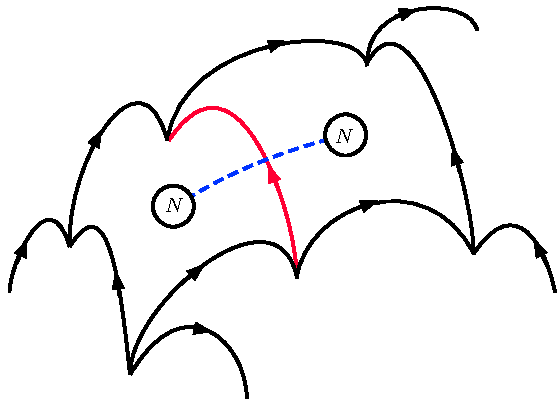
\includegraphics{graph_with_edge_excitation.pdf}
\caption{\label{lattice_w_vortices} A region of the graph $\mcg$ containing two vortex excitations. 
The two punctures hosting the vortex excitations are marked as circles, with the label $N$ denoting their non-bounding spin structure. 
The dashed blue line is the spin structure defect connecting the two punctures.
The edge colored red intersects the spin structure defect and is excited, violating the edge term $D_e$ in the Hamiltonian. 
}
\end{center}
\end{figure}

One can also consider the excitations corresponding to violations of the edge terms 
(note that these will only be present in theories with q-type objects).
If a given state has a $+1$ eigenvalue under an edge term $(1-D_e)$, 
then the fermions traveling across $e$ pick up an additional minus sign relative to the background spin structure.
This is illustrated in Figure \ref{lattice_w_vortices}, where the violated edge $e$ is shown in red, and the two circles marked $N$ denote the vortices created on either side of $e$. 
Diagrammatically we denote the additional minus sign with a branch cut (the dashed line in Figure \ref{lattice_w_vortices}).
% not taken into account by the spin structure data that comes with our handle decomposition.
This implies that violating a single edge term nucleates a pair of vortices (the set of which are in one-to-one correspondence with the non-bounding idempotents of the tube category) on the plaquettes adjacent to the edge $e$ (recall that the plaquette terms are only non-zero in the ground space of the edge and vertex terms).
This means that the vortex excitations can only be separated
at the expense of a linear increase in energy, and so are linearly confined. 
%These two vortex excitations are linked by a spin structure defect line, 
%\kw{defect or branch cut?  defect doesn't seem like the right word}
%\dave{I think both perspectives are natural in some sense.
%Thinking about the wave function, I think it's more natural to call it a branch cut.
%From the point of view of the Hamiltonian it may be more natural to call it a defect (since it has energy/length, and is observable.)
%I'm going to make a comment below.}
%which crosses $e$ transversely. 
%The extra minus sign picked up by fermions when they travel along $e$ is simply 
%the extra minus sign that fermions encounter when they pass over a spin structure defect line. 
%\kw{ditto; also 2x in fig caption}
%This is illustrated in Figure \ref{lattice_w_vortices}, where the violated edge $e$ is shown in red, and the two circles marked $N$ denote the vortex excitations created on either side of $e$. 
%We think of the dashed blue line as the branch cut connecting the two vortex excitations.
% is the spin structure defect line. 

%Continually violating edge terms along a path of neighboring plaquettes results in two well separated vortex excitations.
%These excitations are linked by a spin structure defect line, which excites each edge that it crosses. 
%This means that the vortex excitations can only be separated
%at the expense of a linear increase in energy, and so the vortex excitations are linearly confined. 
%\dave{Note to self: this is only true if the fusino category has q-type objects, 
%otherwise there are no edge terms to violate.}
%added a statement about this

%\ethan{Dave, might want to look at this again. I tried to make the wording something closer to the 
%overlap in our favorite definitions of confinement}
%\dave{First part is very nice. Second part is also nice, but I disagree with the terminology.
%If you have references using that terminology, then please send them to me. 
%Otherwise it is non-standard and I would like to change it, but keep the content roughly the same. 
%Lets Skype about it.} 
%The energetic properties of the vortices depend on how we define the edge term in the Hamiltonian. 
%As written in \eqref{terms_in_ham}, the defect lines (which fermions see as spin structure branch cuts) connecting two vortices have an energy proportional 
%to their length. 
%Alternatively, we can introduce vortices at different locations by requiring some of the plaquettes to have a non-bounding spin structure (if we connect to vortices by spin structure branch cuts, then the $\alpha(e)$ crossing the branch cut will have an additional minus sign relative to the Hamiltonian containing no vortices.).
%one may modify the Hamiltonian to be defined on a graph with some plaquettes inheriting non-bounding 
%spin structures at the locations of the vortices, 
%We must incorporate the vortices effect on the spin structure into the $\alpha(e)$ factors appearing in the expression for $D_e$. 
%\dave{The following sentence I disagree with in a few places -- I made comments. 
%Mostly terminological.
%The content of the sentence is `branch cuts can be moved with guage transformations sending $\Gamma_i \ra - \Gamma_i$ and appropriately taking $\alpha(e) \ra - \alpha(e) $.' }
%Doing this gives the spin structure defect lines zero energy\dave{Why do you call them defect lines? Would you say the BN torus has a defect line?}; they become tensionless \dave{How are you defining string tension? e.g., what's the guage invariant observable you use to measure string tension?} and are free to fluctuate \dave{The branch cut has no dynamics and so cannot fluctuate.} under the action of flat $\zt$ gauge transformations acting on $C^1(\mcg^*)$.
%The vortices are still not truly deconfined\dave{they aren't deconfined at all, see below.} however, since moving them without changing the 
%$\alpha(e)$ factors in the edge term will lead to violations of the edge term. 
%\dave{I disagree. 
%I think you have just defined the Hamiltonian with vortices living at the termination of branch cuts. If you try to move them you will need to violate edge terms as noted in the following sentence.}
%Thus, the vortex excitations themselves are still immobile. 
%\dave{because they are confined.}
%\ethan{no, because if we move them we change the spin structure, but we are keeping the spin structure fixed when we define the hamiltonian. So we can't move them without re-defining the Hamiltonian.}
%\dave{I think it's a terminological issue. Let me explain why I said `because they are confined'. We can Skype about it. 
%Whether or not a `particle' is confined is a property of the phase of matter. 
%I define a deconfined particle to be one that can be brought infinitely far from its partner with finite energy.
%We agree that the Hamiltonian (without vortices put in by hand) has vortices, but they are linearly confined. 
%Now we modify the Hamiltonian by introducing a branch cut which serves to pin vortices at the branch cuts termination. 
%The new Hamiltonian has a two defects in it (the vortices) but is still in the same phase of matter (in particular the vortices are confined). 
%Now given this Hamiltonian, we can ask what's preventing us from moving that `vortex' away from the termination of the branch cut. 
%I would say it cannot move because the vortices are confined. 
%E.g., if we tried to move it we would find a linear cost in energy as the vortex is moved away from the branch cut termination. 
%} 
%To deconfine the vortex defects and allow them to move freely, one needs to make the spin structure dynamical; we leave the study of this possibility to future work. 
%\dave{This last sentence is what I thought the paragraph was supposed to be about.
%Ethan, do you know a good reference for this?}

\dave{Will add comment about how edge terms are modified when we modify spin structure comment on branch cut.}
\dave{Made some edits to this paragraph Ethan and Kevin should probably take a look and make sure they are happy with it.}
\ethan{looks nice! I'm good with it}
Alternatively, by modifying the Hamiltonian we can introduce vortices by hand. 
We remove the plaquette terms where we wish the vortices to reside, 
and require the corresponding plaquettes to have a non-bounding spin structure.
Relative to the un-modified Hamiltonian, 
the vortices will be connected by spin structure branch cuts.
A ground state of the modified Hamiltonian will be an excited state of the un-modified Hamiltonian, 
whose energy depends on the choice of branch cut.
%\dave{I disagree. 
%I think you have just defined the Hamiltonian with vortices living at the termination of branch cuts. If you try to move them you will need to violate edge terms as noted in the following sentence.}
To deconfine the vortices one needs to give the spin structure dynamics; 
we leave the study of this possibility to future work.
\dave{Need to find reference for this last sentence.
I think it may be one of those things that is well known, but not well presented (although I do recall seeing a paper appear on the arxiv that went through this for $p+ip$ but can't find it anymore)}

